% Volume III, Chapter 1 (formerly drafted as Chapter XXVII)
\chapter{Higher-Rank Buildings: The Cubic Trace Identity, Garland Rigidity, and the Hecke Pencil}\label{chap:V3P1}
\chaptermark{Higher-Rank Buildings}
\begin{chapterabstract}
This chapter sets up the topology that the rest of Volume~III uses on $\Atwo$ complexes, with
full proofs where earlier chapters quoted results. Four things are established. First, the
trace mechanism. A diagonal conjugation $D\Cthree D^{-1}=\omega\Cthree$ comes from the $\Z/3$
type grading, and it forces $\Tr(\Cthree)^{k}=0$ for $3\nmid k$. Reading off the diagonal
blocks of $(\Cthree)^{3}$, each as a count of closed walks, gives
$\Tr(\Cthree)^{3}=\Tr A_1^{3}-3q|E|+3nq^{3}$. Under the flag condition this equals
$3|F|-3q|E|+3nq^{3}=n(q-1)^{2}(q+1)$, and the counts $|E|$ and $|F|$ are read off the
point--line flags of $\PG(2,q)$ in the vertex links. In every rank $d$ the same mechanism, with the
partial flags of $\PG(d,q)$ counted by $q$-multinomials, gives
$\Tr(C^{(d+1)})^{d+1}=n\prod_{i=1}^{d}(1-q^{i})$, whose sign is $(-1)^{d}$. Second, Garland rigidity in \emph{local}
form. If every vertex link of a finite two-dimensional complex is the incidence graph of
$\PG(2,q)$ with $q\ge2$, then $H^{1}(Y;\mathcal E)=0$ for \emph{every} unitary local system
$\mathcal E$. The proof is self-contained and uses only the spectral gap
$1-\sqrt q/(q+1)>\tfrac12$ of the link. It needs no building, no free action and no flag
condition, and it therefore covers the complexes of Vol.~I--II, Chapter~\ref{M-chap:X} that fail the flag
condition. Three consequences follow: $b_1=0$, the group $H_1(Y;\Z)$ is finite, and every
unitary representation of $\pi_1(Y)$ is infinitesimally rigid. So no Brillouin zone exists,
abelian or not. Every $\ell$-adic analytic Galois tower over $Y$ has a perfect Lie algebra of
dimension $\ge3$; commutative Iwasawa theory has no rank-two sector, and the smallest possible
Iwasawa algebra is non-commutative. Third, the Hecke pencil. $\det(I-u\Cthree)=\det P(u)$
holds on the nose. The nontrivial eigenvalues of $\DeltaH$ lie in the open right half-plane,
which removes the hypothesis of Vol.~I--II, Theorem~\ref{M-X:thm:hecke}(ii). The factor $(1-u^{3})$ occurs
with multiplicity exactly $b_0=1$, and the exact derivative identity is
$\frac{d}{du}\det(I-u\Cthree)\big|_{u=1}=(-1)^{n}\,n(q-1)^{2}(q+1)\,|\JacH(Y)|$. Under the flag
condition this reads $(-1)^{n}\Tr(\Cthree)^{3}\cdot|\JacH(Y)|$. The factorization
$(1-u^{3})^{b_2-b_1}P(u)$ proposed in the proposed programme is false, by a degree count, and we
say where Betti numbers actually enter. Fourth, the complexes $Y_{21}$ and $Y_{42}$ are
rebuilt from the triangle presentation and every number is checked exactly. The flag part of
$\Tr(\Cthree)^{3}$ is $63$ and $126$, but because the flag condition fails, the true traces
are $651$ and $630$.
\end{chapterabstract}

\section*{Status of the results}

Every numbered statement is proved. The only external inputs, each marked where it is used, are
Lazard's theory of uniform pro-$\ell$ groups (Proposition~\ref{V3P1:prop:fab}(iii)) and
Weil's identification of the tangent space of a representation variety
(Proposition~\ref{V3P1:prop:rigid}(ii)). Nothing in Sections~\ref{V3P1:sec:flags}--\ref{V3P1:sec:garland}
or~\ref{V3P1:sec:pencil} depends on either. The Garland vanishing theorem, quoted in
[Vol.~I--II, Ch.~\ref{M-chap:XII}, Thm.~\ref{M-XII:thm:noabelian}] and [Vol.~I--II, Ch.~\ref{M-chap:Phys1}, Thm.~\ref{M-Phys1:thm:nogo}]
from \cite{Ga,BSw}, is proved here in the local form needed (Theorem~\ref{V3P1:thm:garland}).
All finite identities were machine-checked exactly on complexes rebuilt from scratch
(Table~\ref{V3P1:tab:battery}). Section~\ref{V3P1:sec:scope} records what is open and the
corrections to the proposed programme.

\section{Flags of \texorpdfstring{$\PG(2,q)$}{PG(2,q)} and the counts of an \texorpdfstring{$\Atwo$}{A2} complex}\label{V3P1:sec:flags}

We keep Vol.~I--II, Definition~\ref{M-X:def:a2}: $Y$ has vertex set $V$ ($n=|V|$), edge set $E$ and triangle
set $F$, a type map $\tau\colon V\to\Z/3$, the type-increasing adjacency $A_1$ and $A_2=A_1^{t}$
with $A_1A_2=A_2A_1$. The \emph{link} $\mathrm{Lk}(v)$ is the graph whose vertices are the
neighbours of $v$, with $w\sim x$ when $\{v,w,x\}\in F$. We shall often use the following
purely local hypothesis in place of (ii)--(iii):
\begin{itemize}
\item[(L)] every vertex link $\mathrm{Lk}(v)$ is isomorphic to the point--line incidence graph
$\mathcal I(q)$ of $\PG(2,q)$, the neighbours of type $\tau(v)+1$ going to points and those of
type $\tau(v)+2$ to lines.
\end{itemize}
This is the situation for quotients of thick $\Atwo$ buildings, and it was verified on every
complex of [Vol.~I--II, Ch.~\ref{M-chap:X}] (Heawood links, $q=2$).

\begin{lemma}[Flag counts in $\PG(2,q)$]\label{V3P1:lem:pg}
$\PG(2,q)$ has $q^{2}+q+1$ points and $q^{2}+q+1$ lines. Every line carries $q+1$ points,
every point lies on $q+1$ lines, and two distinct points lie on exactly one line. The number
of flags \textup{(}incident point--line pairs\textup{)} is $(q^{2}+q+1)(q+1)$. Consequently
$\mathcal I(q)$ is a bipartite $(q+1)$-regular graph with $2(q^{2}+q+1)$ vertices and
$(q^{2}+q+1)(q+1)$ edges. For $q=2$ it is the Heawood graph, with $14$ vertices, $21$ edges
and girth $6$.
\end{lemma}

\begin{proof}
Points and lines are the $1$- and $2$-dimensional subspaces of $\F_q^{3}$. There are
$(q^{3}-1)/(q-1)=q^{2}+q+1$ lines through the origin, and by duality ($W\mapsto W^{\perp}$
for the standard bilinear form) the same number of planes. A plane $W\cong\F_q^{2}$ contains
$(q^{2}-1)/(q-1)=q+1$ lines through the origin, and dually a line lies in $q+1$ planes. Two
distinct lines through the origin span exactly one plane. Counting flags by points gives
$(q^{2}+q+1)(q+1)$. The girth of $\mathcal I(q)$ is $6$: there is no $4$-cycle, because two
points share at most one line, and every triangle of the plane gives a $6$-cycle.
\end{proof}

\begin{figure}[t]
\centering
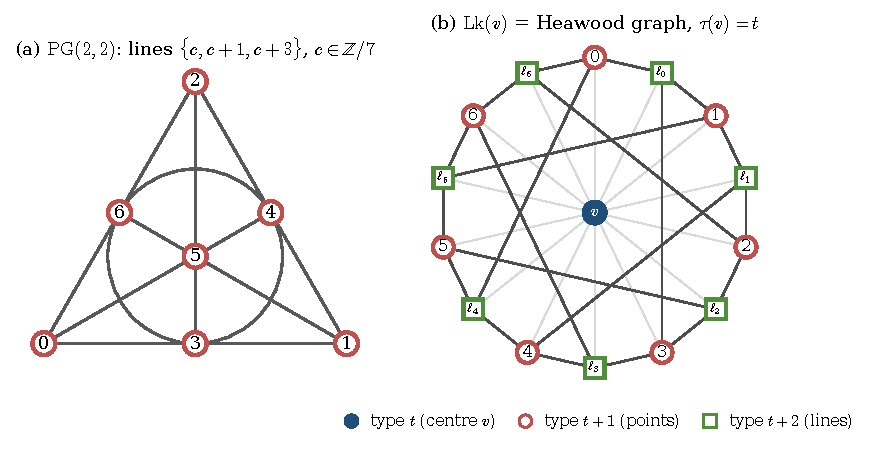
\includegraphics[width=\textwidth]{figures/fig_heawood_fano.pdf}
\caption{The local geometry of the complexes of Vol.~I--II for $q=2$. (a) The Fano plane
$\PG(2,2)$, labelled as in the triangle presentation: its seven lines are the translates
$\{c,c+1,c+3\}$, $c\in\Z/7$, of the Singer difference set $\{0,1,3\}$. (b) The link of a vertex $v$ of
type $t$, which by (L) is the incidence graph of (a), the Heawood graph: its $7$ vertices of type
$t+1$ are the points, its $7$ vertices of type $t+2$ are the lines $\ell_c=\{c,c+1,c+3\}$, and its $21$
edges are the flags, i.e.\ the chambers through $v$ (faint spokes). The three colours are the three
classes of the $\Z/3$ type grading used in Proposition~\ref{V3P1:prop:grading}. Drawn by
\texttt{code/make\_figures.py}.}
\label{V3P1:fig:heawood}
\end{figure}

\begin{lemma}[Counts from the links]\label{V3P1:lem:counts}
Assume \textup{(L)}. Then:
\begin{enumerate}
\item[(a)] $|E|=n(q^{2}+q+1)$, each edge lies in exactly $q+1$ triangles, and
$|F|=\tfrac13\,n(q^{2}+q+1)(q+1)$;
\item[(b)] $\Tr(A_1A_2)=|E|$;
\item[(c)] $\Tr A_1^{3}=3|F|+3s$, where $s\ge0$ is the number of $3$-cycles $x\to y\to z\to
x$ of type-increasing edges whose vertex set is \emph{not} a triangle. So
$\Tr A_1^{3}\ge3|F|$, with equality if and only if the flag condition
\textup{(iv)} of Vol.~I--II, Definition~\ref{M-X:def:a2} holds.
\end{enumerate}
\end{lemma}

\begin{proof}
(a) Count vertex--edge incidences. The edges at $v$ are the vertices of $\mathrm{Lk}(v)$, and
there are $2(q^{2}+q+1)$ of them by Lemma~\ref{V3P1:lem:pg}, so $2|E|=2n(q^{2}+q+1)$. The
triangles through an edge $\{v,w\}$ are the edges of $\mathrm{Lk}(v)$ at $w$, and there are
$q+1$ of them. The triangles at $v$ are the edges of $\mathrm{Lk}(v)$, i.e.\ the flags of
$\PG(2,q)$, so counting vertex--triangle incidences gives
$3|F|=n(q^{2}+q+1)(q+1)$.

(b) Each edge $\{x,y\}$ joins vertices of different types, and exactly one of its two
orientations is type-increasing: if $\tau(y)=\tau(x)+1$ it is $x\to y$, and if
$\tau(y)=\tau(x)+2$ then $\tau(x)=\tau(y)+1$ and it is $y\to x$. Hence $A_1$ has exactly
$|E|$ entries equal to $1$, and $\Tr(A_1A_1^{t})=\sum_{x,y}A_1(x,y)^{2}=|E|$.

(c) $\Tr A_1^{3}$ counts closed walks $x\to y\to z\to x$ of type-increasing edges. Such a walk
visits the three types, so $x,y,z$ are distinct. A triangle $\{a,b,c\}$ with
$\tau=(t,t+1,t+2)$ carries exactly one such cycle, $a\to b\to c\to a$ (the reverse is
type-decreasing), and that cycle contributes three closed walks, one for each starting
point. The remaining closed walks come in cyclic classes of three, one class for each
non-triangle $3$-cycle.
\end{proof}

For $q=2$: $|E|=|F|=7n$, and each vertex sees $14$ edges and $21$ triangles, which are the
$14$ vertices and $21$ edges of the Heawood graph (Figure~\ref{V3P1:fig:heawood}).

\section{The \texorpdfstring{$\Z/3$}{Z/3} grading and the cubic trace identity}\label{V3P1:sec:trace}

\paragraph{The rank-one obstruction.} For a $(q+1)$-regular graph, the companion
$C=\begin{psmallmatrix}T_p&-qI\\ I&0\end{psmallmatrix}$ of the Ihara pencil $1-uT_p+qu^{2}$
satisfies $\Tr C=0$ and
\[
\Tr C^{2}=\Tr T_p^{2}-2qn=n(q+1)-2qn=-n(q-1)<0
\]
[Vol.~I--II, Ch.~\ref{M-chap:II}, Lem.~\ref{M-II:lem:tracecomp}]. The positive term $\Tr T_p^{2}=2|E|$
counts closed walks that return by reversing an edge, and it is beaten by the $-qI$ block,
which is hit twice. By [Vol.~I--II, Ch.~\ref{M-chap:II}, Thm.~\ref{M-II:thm:traceany}] no non-negative
matrix of any size carries this spectrum.

In rank two the companion of the cubic pencil
$P(u)=I-uA_1+qu^{2}A_2-q^{3}u^{3}I$ is
\begin{equation}\label{V3P1:eq:C}
\Cthree=\begin{pmatrix}A_1&-qA_2&q^{3}I\\ I&0&0\\ 0&I&0\end{pmatrix}\in M_{3n}(\Z).
\end{equation}

\begin{proposition}[Grading conjugation]\label{V3P1:prop:grading}
Let $\omega=e^{2\pi i/3}$, $D_1=\operatorname{diag}(\omega^{-\tau(v)})_{v\in V}$ and
$D=\operatorname{diag}(D_1,\ \omega D_1,\ \omega^{2}D_1)$. Then
\[
D_1A_1D_1^{-1}=\omega A_1,\qquad D_1A_2D_1^{-1}=\omega^{2}A_2,\qquad D\,\Cthree D^{-1}=\omega\,\Cthree .
\]
Consequently $\Tr(\Cthree)^{k}=0$ for every $k$ with $3\nmid k$, the spectrum of $\Cthree$
\textup{(}with multiplicities\textup{)} is invariant under multiplication by $\omega$, and
$\det(I-u\Cthree)\in\Z[u^{3}]$.
\end{proposition}

\begin{proof}
$(D_1A_1D_1^{-1})_{xy}=\omega^{\tau(y)-\tau(x)}A_1(x,y)=\omega A_1(x,y)$, because $A_1(x,y)\neq0$
forces $\tau(y)=\tau(x)+1$. Transposing gives $\omega^{-1}=\omega^{2}$ for $A_2$. Write
$D=\operatorname{diag}(d_1D_1,d_2D_1,d_3D_1)$ with $(d_1,d_2,d_3)=(1,\omega,\omega^{2})$.
Block $(i,j)$ of $D\Cthree D^{-1}$ is $d_id_j^{-1}D_1\Cthree_{ij}D_1^{-1}$:
\[
(1,1)\colon\ \omega A_1;\quad
(1,2)\colon\ \omega^{-1}\cdot\omega^{2}(-qA_2)=\omega(-qA_2);\quad
(1,3)\colon\ \omega^{-2}q^{3}I=\omega q^{3}I;\quad
(2,1),(3,2)\colon\ \omega I .
\]
So $D\Cthree D^{-1}=\omega\Cthree$, and therefore $\Tr(\Cthree)^{k}=\omega^{k}\Tr(\Cthree)^{k}$,
which vanishes when $\omega^{k}\neq1$. Similarity of $\Cthree$ and $\omega\Cthree$ gives the
invariance of the spectrum. Then $\det(I-u\Cthree)=\det(I-\omega u\Cthree)$, so only powers
of $u^{3}$ occur.
\end{proof}

\begin{remark}[Walk form of the grading]\label{V3P1:rem:walks}
Every entry of $(\Cthree)^{k}$ is a signed, $q$-weighted sum over words in $A_1$ (one type
step up), $A_2$ (one type step down, i.e.\ two steps up modulo~$3$) and the identity blocks,
which shift the block index but not the vertex. A closed contribution to the trace must
return to its starting vertex, and hence to its starting type. With the block bookkeeping,
the net type change of a word of length $k$ is $\equiv k\pmod 3$. This is the combinatorial
content of $D\Cthree D^{-1}=\omega\Cthree$.
\end{remark}

\begin{theorem}[Cubic trace identity]\label{V3P1:thm:trace}
For every $\Atwo$ complex of order $q$, with or without the flag condition,
\begin{equation}\label{V3P1:eq:trace-general}
\Tr(\Cthree)^{3}=\Tr A_1^{3}-3q\,\Tr(A_1A_2)+3nq^{3}=\Tr A_1^{3}-3q|E|+3nq^{3}.
\end{equation}
Under \textup{(L)} this equals $n(q-1)^{2}(q+1)+3s$, with $s$ as in
Lemma~\ref{V3P1:lem:counts}(c). Under the flag condition,
\begin{equation}\label{V3P1:eq:trace-flag}
\Tr(\Cthree)^{3}=3|F|-3q|E|+3nq^{3}=n(q-1)^{2}(q+1)\ \ge 0,
\end{equation}
with equality if and only if $q=1$.
\end{theorem}

\begin{proof}
Write $\Cthree$ by columns: $\mathrm{col}_1=(A_1,I,0)^{t}$,
$\mathrm{col}_2=(-qA_2,0,I)^{t}$, $\mathrm{col}_3=(q^{3}I,0,0)^{t}$. The rows of $\Cthree$ are
$r_1=(A_1,-qA_2,q^{3}I)$, $r_2=(I,0,0)$ and $r_3=(0,I,0)$. Hence the rows of $(\Cthree)^{2}$
are
\[
r_1\Cthree=\bigl(A_1^{2}-qA_2,\ -qA_1A_2+q^{3}I,\ q^{3}A_1\bigr),\qquad
r_2\Cthree=r_1,\qquad r_3\Cthree=r_2 .
\]
The diagonal blocks of $(\Cthree)^{3}=(\Cthree)^{2}\Cthree$ are
\begin{align*}
\bigl((\Cthree)^{3}\bigr)_{11}&=(A_1^{2}-qA_2)A_1+(-qA_1A_2+q^{3}I)\cdot I+q^{3}A_1\cdot 0\\
&=A_1^{3}-qA_2A_1-qA_1A_2+q^{3}I,\\
\bigl((\Cthree)^{3}\bigr)_{22}&=r_1\cdot\mathrm{col}_2=A_1(-qA_2)+(-qA_2)\cdot0+q^{3}I\cdot I=-qA_1A_2+q^{3}I,\\
\bigl((\Cthree)^{3}\bigr)_{33}&=r_2\cdot\mathrm{col}_3=q^{3}I .
\end{align*}
Summing traces and using $\Tr(A_2A_1)=\Tr(A_1A_2)$ gives \eqref{V3P1:eq:trace-general}.
Each term has a walk meaning. $\Tr A_1^{3}$ counts closed type-increasing $3$-walks.
$\Tr(A_1A_2)=|E|$ counts the backtracking $2$-walks $x\to y\leftarrow x$; it enters three
times, once for each of the three cyclic positions at which the backtrack can sit inside a
$3$-step return, each with weight $-q$. The term $q^{3}$ is the pure constant term, entering
once per block. Under (L), Lemma~\ref{V3P1:lem:counts} gives $\Tr A_1^{3}=3|F|+3s$, and
\begin{align*}
3|F|-3q|E|+3nq^{3}
&=n\bigl[(q^{2}+q+1)(q+1)-3q(q^{2}+q+1)+3q^{3}\bigr]\\
&=n\bigl[(q^{3}+2q^{2}+2q+1)-(3q^{3}+3q^{2}+3q)+3q^{3}\bigr]\\
&=n\,(q^{3}-q^{2}-q+1)=n(q-1)^{2}(q+1).
\end{align*}
Under the flag condition $s=0$. The factor $(q-1)^{2}(q+1)$ vanishes only at $q=1$.
\end{proof}

\begin{remark}[Parity versus $\Z/3$]\label{V3P1:rem:parity}
In rank one a closed walk can return in two steps, so the negative block $-qI$ is felt
already at $k=2$, and it is felt twice. In rank two the grading makes $\Tr(\Cthree)^{k}$
blind to everything for $k=1,2$. At $k=3$ the chamber term $3|F|=n(q^{2}+q+1)(q+1)$, the flag
count of $\PG(2,q)$ times $n$, dominates the backtracking loss $3q|E|-3nq^{3}$. The
difference is exactly $n(q-1)^{2}(q+1)$. This is the proof behind
[Vol.~I--II, Ch.~\ref{M-chap:X}, Thm.~\ref{M-X:thm:notrace}], written out in full, and its consequence for
realizability is recorded in [Vol.~I--II, Ch.~\ref{M-chap:X}, Thm.~\ref{M-X:thm:realizable}].
\end{remark}

% Volume III, Chapter 1 -- addendum: the first nonzero trace of the PGL_{d+1} companion on
% A~_d complexes (open problem (a) of Remark V3P1:rem:scope).  Verified by code/v3p1_ad_trace.py.
\section{The first nonzero trace in every rank}\label{V3P1:sec:tracead}

This section settles open problem (a) of Remark~\ref{V3P1:rem:scope}: the value of the first
nonzero trace $\Tr(C^{(d+1)})^{d+1}$ on $\Atilde d$ complexes. The answer is
$n\prod_{i=1}^{d}(1-q^{i})$ under the $\Atilde d$ flag condition, which contains the rank-one value
$-n(q-1)$ and Theorem~\ref{V3P1:thm:trace} as the cases $d=1,2$.

\paragraph{Setting.} An $\Atilde d$ complex $Y$ has a type map $\tau\colon V\to\Z/(d+1)$, and for
$1\le j\le d$ we let $A_j$ be the $0/1$ matrix with $A_j(x,y)=1$ iff $\{x,y\}$ is an edge and
$\tau(y)=\tau(x)+j$; put $A_{d+1}=I$. The local hypothesis replacing (L) is
\begin{itemize}
\item[(L$_d$)] the link of every vertex $v$ is isomorphic to the flag complex of $\PG(d,q)$, the
neighbours of type $\tau(v)+i$ going to the subspaces of codimension $i$ in $\F_q^{d+1}$
($1\le i\le d$), adjacency in the link being containment. By the duality $U\mapsto U^{\perp}$ one
may equally send them to the subspaces of dimension $i$; for $d=2$ that is \textup{(L)}.
\end{itemize}
A \emph{closed walk of increments} $\mathbf j=(j_1,\dots,j_r)$, $j_i\ge1$, is a sequence
$x_0\to x_1\to\dots\to x_r=x_0$ with $A_{j_i}(x_{i-1},x_i)=1$ (the identity step for $j_i=d+1$). The
\emph{flag condition} of rank $d$ is
\begin{itemize}
\item[(F$_d$)] every closed walk whose increments sum to $d+1$ has all its vertices in one simplex.
\end{itemize}
For $d=2$ the only increments with sum $3$ are $(1,1,1)$, $(1,2)$, $(2,1)$ and $(3)$, and (F$_2$) is the
flag condition of Lemma~\ref{V3P1:lem:counts}(c). The companion is
\[
C^{(d+1)}=\begin{pmatrix}
R_1&R_2&\cdots&R_d&R_{d+1}\\ I&0&\cdots&0&0\\ &\ddots&&&\vdots\\ 0&\cdots&&I&0\end{pmatrix},
\qquad R_j=(-1)^{j-1}q^{\binom j2}A_j ,
\]
which is \eqref{V3P1:eq:C} for $d=2$. When the $A_j$ commute, $\det(xI-C^{(d+1)})=\sum_{j=0}^{d+1}(-1)^{j}
q^{\binom j2}A_jx^{d+1-j}$, the local Hecke polynomial of $\PGL_{d+1}$; the companion of
[Vol.~I--II, Ch.~\ref{M-chap:XX}, Thm.~\ref{M-XX:thm:hecke}] has the same excursion weights $R_j$
(see the proof of Lemma~\ref{V3P1:lem:excursion}), hence the same traces of all powers. With
$D_1=\operatorname{diag}(\zeta^{-\tau})$, $\zeta=e^{2\pi i/(d+1)}$, the proof of
Proposition~\ref{V3P1:prop:grading} gives $DC^{(d+1)}D^{-1}=\zeta C^{(d+1)}$ verbatim, so
$\Tr(C^{(d+1)})^{k}=0$ for $(d+1)\nmid k$.

\begin{lemma}[Excursion expansion]\label{V3P1:lem:excursion}
For every $k\ge1$, with no commutativity assumption,
\[
\Tr\bigl(C^{(d+1)}\bigr)^{k}=\sum_{\mathbf j}\,j_1\,(-1)^{k-r}\,q^{\sum_i\binom{j_i}2}\,
\Tr\bigl(A_{j_1}A_{j_2}\cdots A_{j_r}\bigr),
\]
the sum over the compositions $\mathbf j=(j_1,\dots,j_r)$ of $k$ with all parts $\le d+1$.
\end{lemma}

\begin{proof}
$\bigl((C^{(d+1)})^{k}\bigr)_{bb}$ is a sum over closed walks of length $k$ in the graph on the block
indices $1,\dots,d+1$ whose arcs are $1\to j$ (weight $R_j$) and $i+1\to i$ (weight $I$). From block
$1$, the arc $1\to j$ must be followed by $j\to j-1\to\dots\to1$, so every return to block $1$ is an
\emph{excursion} of length $j$ and weight $R_j$. A closed walk of length $k$ is therefore a cyclic
sequence of excursions of lengths $j_1,\dots,j_r$ with $\sum j_i=k$, together with the time at which
it starts. Label the excursions so that the walk starts inside the first one; there are $j_1$ such
starting times, and each contributes the trace of a cyclic rotation of $R_{j_1}\cdots R_{j_r}$, which
is $\Tr(R_{j_1}\cdots R_{j_r})$. Finally $\prod_i(-1)^{j_i-1}=(-1)^{k-r}$. For the companion of
[Vol.~I--II, Ch.~\ref{M-chap:XX}], whose row $0$ carries $q^{i}A_{i+1}$ and whose subdiagonal carries
$-q^{i}I$, an excursion of length $j$ has weight
$q^{j-1}A_j\prod_{l=0}^{j-2}(-q^{l})=(-1)^{j-1}q^{\binom j2}A_j=R_j$. Line (W) checks the expansion
as an identity of non-commutative polynomials for $d\le6$, $k\le d+1$.
\end{proof}

\begin{lemma}[Closed walks are flags]\label{V3P1:lem:flagwalks}
Let $\mathbf j$ be a composition of $d+1$ and let $\binom{d+1}{\mathbf j}_q=[d+1]_q!/\prod_i[j_i]_q!$ be
the $q$-multinomial coefficient, $[k]_q=1+q+\dots+q^{k-1}$.
\begin{enumerate}
\item[(i)] Under \textup{(L$_d$)}, $\Tr(A_{j_1}\cdots A_{j_r})=n\binom{d+1}{\mathbf j}_q+s_{\mathbf j}$,
where $s_{\mathbf j}\ge0$ is the number of closed walks of increments $\mathbf j$ whose vertices are not
contained in one simplex. Under \textup{(F$_d$)}, $s_{\mathbf j}=0$.
\item[(ii)] The Bruhat--Tits building of $\PGL_{d+1}$ over a non-archimedean local field with
residue field $\F_q$ satisfies \textup{(L$_d$)} and \textup{(F$_d$)}.
\end{enumerate}
\end{lemma}

\begin{proof}
(i) A closed walk of increments $\mathbf j$ starting at $x_0$ whose vertices lie in a simplex is
determined by $x_1,\dots,x_{r-1}$, which have types $\tau(x_0)+j_1+\dots+j_i$ and form a simplex of
$\mathrm{Lk}(x_0)$, i.e.\ by (L$_d$) a chain $\F_q^{d+1}\supsetneq U_1\supsetneq\dots\supsetneq
U_{r-1}\supsetneq0$ with $\operatorname{codim}(U_i\subset U_{i-1})=j_i$. Conversely every such chain gives
such a walk, the last step $x_{r-1}\to x_0$ having increment $j_r$. The number of chains is the
$q$-multinomial coefficient (choose $U_{r-1}$, then $U_{r-2}\supset U_{r-1}$, and so on), whatever the
order of the parts. The remaining closed walks are counted by $s_{\mathbf j}$.

(ii) The vertices are the homothety classes of lattices $L\subset K^{d+1}$, with uniformizer
$\pi$; $[L]\to[L']$ has increment $j$ iff there are representatives with $L\supset L'\supset\pi L$ and
$\dim L/L'=j$, and the simplices are the chains of such lattices. The link of $[L]$ is the flag complex
of $L/\pi L\cong\F_q^{d+1}$. Given a closed walk $x_0\to\dots\to x_r=x_0$ with increments summing to
$d+1$, choose $L_0$ in $x_0$ and inductively the unique representative $L_i$ of $x_i$ with
$L_{i-1}\supset L_i\supset\pi L_{i-1}$. Then $[L_0:L_r]=q^{d+1}$ and $L_r$ is homothetic to $L_0$,
so $L_r=\pi L_0$. Hence $L_0\supset L_1\supset\dots\supset L_{r-1}\supset\pi L_0$ is a chain, and the
vertices of the walk span a simplex.
\end{proof}

\begin{theorem}[First nonzero trace in rank $d$]\label{V3P1:thm:tracead}
Let $Y$ be a finite $\Atilde d$ complex satisfying \textup{(L$_d$)}, with $n$ vertices. Then
$\Tr(C^{(d+1)})^{k}=0$ for $(d+1)\nmid k$, and
\[
\Tr\bigl(C^{(d+1)}\bigr)^{d+1}=n\prod_{i=1}^{d}\bigl(1-q^{i}\bigr)
+\sum_{\mathbf j}j_1(-1)^{d+1-r}q^{\sum_i\binom{j_i}2}s_{\mathbf j}.
\]
Under the flag condition \textup{(F$_d$)},
\[
\Tr\bigl(C^{(d+1)}\bigr)^{d+1}=n\prod_{i=1}^{d}\bigl(1-q^{i}\bigr)=(-1)^{d}\,n\,(q-1)^{d}\,[d]_q!\,.
\]
For $d=1,2,3,4$ this is $-n(q-1)$, $n(q-1)^{2}(q+1)$, $-n(q-1)^{3}(q+1)(q^{2}+q+1)$ and
$n(q-1)^{4}(q+1)^{2}(q^{2}+1)(q^{2}+q+1)$.
\end{theorem}

\begin{proof}
By Lemmas~\ref{V3P1:lem:excursion} and~\ref{V3P1:lem:flagwalks} it remains to show, with $m=d+1$,
\[
T_m:=\sum_{\mathbf j\models m}j_1(-1)^{m-r}q^{\sum\binom{j_i}2}\binom{m}{\mathbf j}_q=\prod_{i=1}^{m-1}(1-q^{i}).
\]
Write $\binom{m}{\mathbf j}_q=[m]_q!\prod_iE_{j_i}$ with $E_j=q^{\binom j2}/[j]_q!$ and work in
$\Z[[q]][[t]]$. Put $F(t)=\sum_{j\ge1}(-1)^{j-1}E_jt^{j}$. Expanding $tF'(t)/(1-F(t))$ by the geometric
series gives $\sum_{\mathbf j}j_1\prod_i(-1)^{j_i-1}E_{j_i}t^{\sum j_i}$, the $j_1$ coming from the
derivative applied to the first factor; hence $T_m=[m]_q!\,[t^{m}]\bigl(-t\tfrac{d}{dt}\log(1-F(t))\bigr)$.
Now $1-F(t)=\sum_{j\ge0}q^{\binom j2}(-t)^{j}/[j]_q!$, and since $[j]_q!=(q;q)_j/(1-q)^{j}$, Euler's
identity $\sum_jq^{\binom j2}z^{j}/(q;q)_j=\prod_{i\ge0}(1+zq^{i})$ with $z=-(1-q)t$ gives
$1-F(t)=\prod_{i\ge0}\bigl(1-(1-q)q^{i}t\bigr)$. Therefore
\[
-t\frac{d}{dt}\log(1-F(t))=\sum_{i\ge0}\frac{(1-q)q^{i}t}{1-(1-q)q^{i}t}
=\sum_{k\ge1}t^{k}\,(1-q)^{k}\sum_{i\ge0}q^{ik}=\sum_{k\ge1}t^{k}\frac{(1-q)^{k}}{1-q^{k}},
\]
and $T_m=[m]_q!\,(1-q)^{m}/(1-q^{m})=\prod_{i=1}^{m}(1-q^{i})/(1-q^{m})=\prod_{i=1}^{m-1}(1-q^{i})$.
Both sides are polynomials in $q$, so the identity in $\Z[[q]]$ is an identity of polynomials. The
last form uses $1-q^{i}=-(q-1)[i]_q$.
\end{proof}

\begin{corollary}\label{V3P1:cor:tracead}
Assume \textup{(L$_d$)} and \textup{(F$_d$)}.
\begin{enumerate}
\item[(i)] As a polynomial in $q$, $\Tr(C^{(d+1)})^{d+1}/n$ vanishes at $q=1$ to order exactly $d$. A
thin complex ($q=1$) satisfying \textup{(F$_d$)} has $\Tr(C^{(d+1)})^{d+1}=0$.
\item[(ii)] For $q\ge2$ the sign of $\Tr(C^{(d+1)})^{d+1}$ is $(-1)^{d}$. For odd $d$ it is negative, so
no non-negative matrix, of any size, has the nonzero spectrum of $C^{(d+1)}$ (with multiplicities):
the obstruction of the rank-one paragraph of Section~\ref{V3P1:sec:trace} recurs in every odd rank,
and disappears in every even rank.
\item[(iii)] On the constants, $A_j$ acts by $\binom{d+1}j_q$ and the local factor is
$\prod_{i=0}^{d}(1-q^{i}u)$; its derivative at $u=1$ is $-\prod_{i=1}^{d}(1-q^{i})$. So the coincidence
of Remark~\ref{V3P1:rem:coincidence} persists in every rank: the first nonzero trace per vertex and the
derivative of the trivial local factor at $u=1$ are the same number up to sign.
\end{enumerate}
\end{corollary}

\begin{proof}
(i) Each factor $1-q^{i}$ has a simple zero at $q=1$. (ii) Each factor is negative for $q\ge2$. The
traces of the powers of a non-negative matrix are non-negative, and padding by zeros does not change
them. (iii) $\sum_j(-1)^{j}q^{\binom j2}\binom{d+1}j_qx^{d+1-j}=\prod_{i=0}^{d}(x-q^{i})$ by the
$q$-binomial theorem, and differentiate.
\end{proof}

\begin{remark}[Numerical record]\label{V3P1:rem:traceadnum}
\texttt{code/v3p1\_ad\_trace.py} (numpy, scipy, sympy; about two minutes) checks: the excursion
expansion as non-commutative words (W); the identity $T_m=\prod_{i<m}(1-q^{i})$ symbolically for
$d\le12$, the order of the zero at $q=1$ and the sign (Q); the chain counts in $\F_q^{d+1}$ by
enumeration of all subspaces for $(d,q)=(2,2),(3,2),(2,3),(3,3),(4,2)$, with per-vertex traces $3$,
$-21$, $16$, $-416$, $315$ (F); the thin $\Atilde d$ tori $(\Z/m)^{d+1}/\Z(1,\dots,1)$ for $d=2,3,4$, which
satisfy \textup{(F$_d$)} for $m\ge d+2$ and give $\Tr(C^{(d+1)})^{d+1}=0$ there, while for $m=d+1$ the
excess walks of increments $(1,\dots,1)$ give $\Tr=(d+1)n$ (T); and $Y_{21}$, where
$651=63+3\cdot196$ (Y). No finite thick $\Atilde3$ complex is constructed; for $d\ge3$ the thick case
rests on Lemma~\ref{V3P1:lem:flagwalks}(ii) and on the per-vertex count (F).
\end{remark}

\begin{remark}[Corrections to the proposed programme]\label{V3P1:rem:traceadcorr}
(1) The proposed $\Tr(C^{(4)})^{4}=n(q-1)^{3}(q+1)(q^{2}+1)$ is false: the value is
$-n(q-1)^{3}(q+1)(q^{2}+q+1)$, e.g.\ $-21n$ instead of $15n$ at $q=2$; the sign is negative and the
last factor is $[3]_q$, not $q^{2}+1$. (2) The proposed general form
$n(q-1)^{d}\prod_j(q^{j+1}-1)/(q-1)$ is false; the correct product is $(-1)^{d}n(q-1)^{d}[d]_q!$. (3) For
$d\ge3$ the trace is not a combination of the cell numbers $|F_k|$ alone: the words $A_{j_1}\cdots
A_{j_r}$ count partial flags of every type, which is why the $q$-multinomials enter. (4) The vertex
block of $L_E$ for $d\ge3$ (Chapter~\ref{chap:V3P4}, Remark~\ref{V3P4:rem:scope}(a)) is a different problem and is not
addressed here.
\end{remark}


\section{Garland rigidity by the local spectral gap}\label{V3P1:sec:garland}

\paragraph{Unitary local systems.} A rank-$N$ unitary local system $\mathcal E$ on a finite
simplicial complex $Y$ is given by a Hermitian space $\mathcal E_v\cong\C^{N}$ at each vertex
and a unitary transport $g_{uv}\colon\mathcal E_v\to\mathcal E_u$ for each oriented edge, with
$g_{vu}=g_{uv}^{-1}$ and $g_{ab}g_{bc}=g_{ac}$ on every triangle (flatness). Equivalently, it
is a representation $\rho\colon\pi_1(Y)\to U(N)$ up to conjugation, and the trivial system
$\mathcal E=\C$ gives ordinary cohomology. Cochains are
\[
C^{0}=\{\varphi(v)\in\mathcal E_v\},\quad
C^{1}=\{f(u,v)\in\mathcal E_u:\ f(v,u)=-g_{vu}f(u,v)\},
\]
and $C^{2}$ consists of alternating functions on oriented triangles with values in the fibre
at the first vertex. The differentials are
\[
(\delta\varphi)(u,v)=g_{uv}\varphi(v)-\varphi(u),\qquad
(\delta f)(a,b,c)=f(a,b)+g_{ab}f(b,c)+g_{ac}f(c,a).
\]
Flatness gives $\delta\delta=0$:
$(\delta\delta\varphi)(a,b,c)=g_{ab}g_{bc}\varphi(c)-g_{ac}\varphi(c)=0$.

\paragraph{Weights.} Let $m(e)$ be the number of triangles containing the edge $e$, and
$m(v)=\sum_{w\sim v}m(vw)$. We put
\[
\langle\varphi,\psi\rangle=\sum_vm(v)\langle\varphi(v),\psi(v)\rangle,\qquad
\langle f,h\rangle=\tfrac12\sum_{(u,v)}m(uv)\langle f(u,v),h(u,v)\rangle,
\]
where the second sum is over oriented edges. It is well defined because transport is unitary.
Under (L), $m(e)=q+1$ and $m(v)=2(q+1)(q^{2}+q+1)$ are constant, so these are scalar multiples
of the standard inner products, and the harmonic forms below are the standard ones.

\begin{lemma}[Adjoint and Hodge]\label{V3P1:lem:adjoint}
$(\delta^{*}f)(u)=-\frac1{m(u)}\sum_{v\sim u}m(uv)f(u,v)$, and
$H^{1}(Y;\mathcal E)\cong\ker\delta\cap\ker\delta^{*}\subseteq C^{1}$.
\end{lemma}

\begin{proof}
Start from $\langle\delta\varphi,f\rangle=\tfrac12\sum_{(u,v)}m(uv)\bigl(\langle g_{uv}\varphi(v),
f(u,v)\rangle-\langle\varphi(u),f(u,v)\rangle\bigr)$. By unitarity and antisymmetry,
$\langle g_{uv}\varphi(v),f(u,v)\rangle=\langle\varphi(v),g_{vu}f(u,v)\rangle
=-\langle\varphi(v),f(v,u)\rangle$. Relabelling $(u,v)\leftrightarrow(v,u)$ turns the first
sum into the second, so $\langle\delta\varphi,f\rangle=-\sum_{(u,v)}m(uv)\langle\varphi(u),
f(u,v)\rangle$, which is the stated adjoint. Since $C^{1}=\operatorname{im}\delta\oplus
(\operatorname{im}\delta)^{\perp}$ and $(\operatorname{im}\delta)^{\perp}=\ker\delta^{*}$,
every class in $\ker\delta/\operatorname{im}\delta$ has a unique representative in
$\ker\delta\cap\ker\delta^{*}$.
\end{proof}

\begin{lemma}[Spectrum of the link]\label{V3P1:lem:gap}
The adjacency eigenvalues of $\mathcal I(q)$ are $\pm(q+1)$, each simple, and $\pm\sqrt q$,
each with multiplicity $q^{2}+q$. The normalized Laplacian $I-\frac1{q+1}\mathrm{Adj}$
therefore has smallest positive eigenvalue
\[
\lambda(q)=1-\frac{\sqrt q}{q+1},\qquad\text{and}\qquad 2\lambda(q)-1=\frac{(\sqrt q-1)^{2}}{q+1}.
\]
So $\lambda(q)>\tfrac12$ for every $q\ge2$ and $\lambda(1)=\tfrac12$. For the Heawood graph,
$\lambda(2)=1-\sqrt2/3=0.528595\ldots$
\end{lemma}

\begin{proof}
Let $N$ be the point--line incidence matrix. By Lemma~\ref{V3P1:lem:pg},
$NN^{t}=(q+1)I+(J-I)=qI+J$, since a point lies on $q+1$ lines and two points share one line.
Its eigenvalues are $q+(q^{2}+q+1)=(q+1)^{2}$ on $\mathbf 1$ and $q$ on $\mathbf 1^{\perp}$.
The adjacency $\begin{psmallmatrix}0&N\\N^{t}&0\end{psmallmatrix}$ has eigenvalues
$\pm\sqrt{\,\cdot\,}$ of these, and the graph is $(q+1)$-regular. The simplicity of $q+1$
shows that $\mathcal I(q)$ is connected.
\end{proof}

For a $\mathcal E_v$-valued function $\phi$ on $\mathrm{Lk}(v)$ put
$\|\phi\|^{2}_{v}=\sum_{w}m(vw)|\phi(w)|^{2}$ and $\|d\phi\|^{2}_{v}=\sum_{\{w,x\}}|\phi(x)-\phi(w)|^{2}$,
the second sum running over link edges, i.e.\ over triangles $\{v,w,x\}$. The degree of $w$
in $\mathrm{Lk}(v)$ is $m(vw)$. So if $\sum_wm(vw)\phi(w)=0$, then
$\|d\phi\|_v^{2}\ge\lambda(q)\|\phi\|_v^{2}$, applying Lemma~\ref{V3P1:lem:gap} componentwise
in an orthonormal basis of $\mathcal E_v$.

\begin{theorem}[Garland vanishing, local form]\label{V3P1:thm:garland}
Let $Y$ be a finite two-dimensional simplicial complex satisfying \textup{(L)} with $q\ge2$.
No building, free action or flag condition is assumed. Then $H^{1}(Y;\mathcal E)=0$ for every
unitary local system $\mathcal E$ on $Y$. In particular:
\begin{enumerate}
\item[(i)] $b_1(Y;\R)=b_1(Y;\C)=0$, and $H_1(Y;\Z)$ is a finite abelian group;
\item[(ii)] $\coker_\Z\Delta_1=\Jac_1(Y)$, i.e.\ the edge critical group is the whole cokernel;
the group $K(Y)=\ker\partial_1/\operatorname{im}(\partial_2\partial_2^{t})$ is finite and
surjects onto $H_1(Y;\Z)$; and $b_2=\chi(Y)-1$;
\item[(iii)] every finite connected cover $Y'\to Y$ satisfies \textup{(L)}, hence (i)--(ii).
\end{enumerate}
\end{theorem}

\begin{proof}
Let $f\in\ker\delta\cap\ker\delta^{*}$ (Lemma~\ref{V3P1:lem:adjoint}). For each vertex $v$
define the localization $f_v(w):=f(v,w)\in\mathcal E_v$ for $w\in\mathrm{Lk}(v)$. All of its
values lie in the \emph{single} fibre $\mathcal E_v$, so no trivialization is needed. We prove
three identities.

\emph{(a) Mass.} $\sum_v\|f_v\|_v^{2}=\sum_v\sum_{w\sim v}m(vw)|f(v,w)|^{2}
=\sum_{(v,w)}m(vw)|f(v,w)|^{2}=2\|f\|^{2}$.

\emph{(b) Energy.} Fix a triangle $\{a,b,c\}$; it is the link edge $\{b,c\}$ of
$\mathrm{Lk}(a)$. Since $\delta f=0$ and $g_{ac}f(c,a)=-f(a,c)$,
\[
f_a(c)-f_a(b)=f(a,c)-f(a,b)=g_{ab}f(b,c),\qquad\text{so}\qquad |f_a(c)-f_a(b)|=|f(b,c)|.
\]
Summing over the three vertices of every triangle,
$\sum_v\|df_v\|_v^{2}=\sum_{\{a,b,c\}\in F}\bigl(|f(b,c)|^{2}+|f(c,a)|^{2}+|f(a,b)|^{2}\bigr)
=\sum_{e}m(e)|f(e)|^{2}=\|f\|^{2}$.

\emph{(c) Balance.} $\sum_{w}m(vw)f_v(w)=-m(v)(\delta^{*}f)(v)=0$.

By (c) and Lemma~\ref{V3P1:lem:gap}, $\|df_v\|_v^{2}\ge\lambda(q)\|f_v\|_v^{2}$ for every $v$.
Summing and using (a) and (b),
\[
\|f\|^{2}=\sum_v\|df_v\|_v^{2}\ \ge\ \lambda(q)\sum_v\|f_v\|_v^{2}=2\lambda(q)\|f\|^{2},
\qquad\text{i.e.}\qquad \frac{(\sqrt q-1)^{2}}{q+1}\,\|f\|^{2}\le0 .
\]
Hence $f=0$ for $q\ge2$. For (i), take $\mathcal E$ trivial: $H^{1}(Y;\C)=0$, so $b_1=0$, and
$H_1(Y;\Z)$ is finitely generated of rank $0$. For (ii), $\coker\Delta_1\cong\Z^{b_1}\oplus
\Jac_1(Y)$ by Vol.~I--II, Proposition~\ref{M-X:prop:hodge}. $K(Y)$ has rank $\rank\ker\partial_1-
\rank\partial_2=b_1=0$, and it surjects onto $\ker\partial_1/\operatorname{im}\partial_2=
H_1(Y;\Z)$ because $\operatorname{im}(\partial_2\partial_2^{t})\subseteq\operatorname{im}
\partial_2$. Finally $\chi=b_0-b_1+b_2$. For (iii), links are local, and a covering map is a
simplicial isomorphism on stars.
\end{proof}

\begin{remark}[Sharpness and provenance]\label{V3P1:rem:sharp}
At $q=1$ the link is the hexagon, $2\lambda(1)-1=0$, and the inequality is empty. The thin
tori of Vol.~I--II, Construction~\ref{M-X:con:thin} indeed have $b_1=2$, so the threshold
$\lambda>\tfrac12$ is exactly where rank two separates from flat. The argument is Garland's
local-to-global method \cite{Ga}, in the form isolated by Ballmann--\'Swi\k{a}tkowski
\cite{BSw} and \.Zuk \cite{Zuk96}. We have written it for unitary local systems because this
costs nothing and gives Proposition~\ref{V3P1:prop:rigid}. It sharpens
[Vol.~I--II, Ch.~\ref{M-chap:XII}, Thm.~\ref{M-XII:thm:noabelian}] in two respects: no group action is used,
and the flag condition is not needed. The latter matters because four of the five complexes
of [Vol.~I--II, Ch.~\ref{M-chap:X}] violate it.
\end{remark}

\begin{remark}[Correction to {[Vol.~I--II, Ch.~\ref{M-chap:Phys1}, Rem.~\ref{M-Phys1:rem:global}]}]\label{V3P1:rem:physcorr}
That remark asserts that ``no local inspection of a rank-two hyperbolic lattice reveals the
obstruction''. Theorem~\ref{V3P1:thm:garland} shows the opposite for $b_1$. The vanishing of
$b_1$ is certified by the vertex links alone, through the single number
$\lambda(2)=1-\sqrt2/3>\tfrac12$ of the Heawood graph. What is genuinely global is the finite
group $H_1(Y;\Z)$ itself, e.g.\ $(\Z/2)^{6}$ versus $(\Z/2)^{3}\oplus(\Z/4)^{2}$ for two
complexes with identical links, and property (T) of $\pi_1(Y)$.
\end{remark}

\begin{remark}[$\Atilde d$, $d\ge3$]\label{V3P1:rem:Ad}
Since $H^{1}$ depends only on the $2$-skeleton, the proof above applies to an $\Atilde d$
complex as soon as the $1$-skeleton of each vertex link (the spherical building of $\PG(d,q)$,
weighted by triangle counts) has normalized spectral gap $>\tfrac12$. We have not computed that
gap for $d\ge3$, and we do not claim it. For thick $\Atilde d$ buildings with $d\ge3$,
$b_1=0$ of finite free quotients follows instead from Tits' theorem that such buildings are
Bruhat--Tits and from Kazhdan's property (T) for simple groups of rank $\ge2$ over local
fields. These are quoted, not proved here, and nothing below uses them.
\end{remark}

\section{What rigidity removes: Brillouin zones, abelian towers, and the non-commutative turn}\label{V3P1:sec:turn}

\begin{proposition}[No continuous character families]\label{V3P1:prop:rigid}
Let $Y$ satisfy \textup{(L)} with $q\ge2$.
\begin{enumerate}
\item[(i)] $\Hom(\pi_1(Y),U(1))=\Hom(H_1(Y;\Z),U(1))$ is a finite group, isomorphic to
$H_1(Y;\Z)$. For every $\chi$ in it, $H^{1}(Y;\C_\chi)=0$.
\item[(ii)] For every unitary $\rho\colon\pi_1(Y)\to U(N)$, $H^{1}(\pi_1(Y);\mathfrak{gl}_N(\C)_{\mathrm{Ad}\rho})=0$.
Hence, by Weil's criterion, every first-order deformation of $\rho$ in
$\Hom(\pi_1(Y),\GL_N(\C))$ is tangent to its conjugation orbit: unitary representations are
infinitesimally rigid, and the unitary character variety has no positive-dimensional
component through any point.
\end{enumerate}
\end{proposition}

\begin{proof}
(i) $U(1)$ is abelian, $H_1(Y;\Z)$ is finite (Theorem~\ref{V3P1:thm:garland}), and a finite
abelian group is isomorphic to its Pontryagin dual. Then apply Theorem~\ref{V3P1:thm:garland}
to the rank-one system $\C_\chi$. (ii) $\mathrm{Ad}\rho$ preserves the Hilbert--Schmidt
product $\operatorname{tr}(X^{*}Y)$, so it defines a unitary local system of rank $N^{2}$. In
degree one, $H^{1}(\pi_1(Y);V)=H^{1}(Y;\mathcal V)$ for any connected CW complex. Apply
Theorem~\ref{V3P1:thm:garland}. Weil's criterion \cite{Wei64} identifies the Zariski tangent
space of the representation variety at $\rho$ with the cocycles $Z^{1}(\pi_1(Y);
\mathfrak{gl}_N)$, and the tangent space to the orbit with the coboundaries.
\end{proof}

\begin{remark}[Brillouin zones]\label{V3P1:rem:bz}
Bloch--Floquet theory for a $\Z^{d}$-periodic operator decomposes it over the torus
$\widehat{\Z^{d}}=\Hom(\Z^{d},U(1))$, the Brillouin zone. For a periodic operator on the
maximal abelian cover of $Y$ (Hecke operators, the Hodge Laplacians, or any tight-binding
Hamiltonian), the same decomposition runs over $\Hom(H_1(Y;\Z),U(1))$. By
Proposition~\ref{V3P1:prop:rigid}(i) this is a \emph{finite} set of $|H_1(Y;\Z)|$ points, and
the Bloch decomposition is a finite direct sum of twisted operators: $64$ of them for $Y_{21}$
and $128$ for $Y_{42}$ (Section~\ref{V3P1:sec:examples}). There is no continuous momentum, and
therefore no band, group velocity or effective mass. Part~(ii) says more: no continuous
family of \emph{non-abelian} unitary twists exists either, even infinitesimally. This is the
precise content of ``the Brillouin zone is erased'', and it strengthens
[Vol.~I--II, Ch.~\ref{M-chap:Phys1}, Thm.~\ref{M-Phys1:thm:nogo}]. That theorem obtained (iv) from property
(T) of the group; here the rigidity is derived from the links.
\end{remark}

\begin{proposition}[Galois towers over $Y$]\label{V3P1:prop:fab}
Let $Y$ satisfy \textup{(L)} with $q\ge2$, and let $G$ be the profinite Galois group of a tower
of finite connected Galois covers $(Y_U)_U$ of $Y$, indexed by the open normal subgroups
$U\le G$.
\begin{enumerate}
\item[(i)] Every open subgroup $U\le G$ has finite abelianization
$U^{\mathrm{ab}}=U/\overline{[U,U]}$.
\item[(ii)] In particular no open subgroup of $G$ surjects onto $\Z_\ell$. There are no
$\Z_\ell$-towers, and no $\Z_\ell^{r}$-towers for any $r\ge1$, over any finite cover of $Y$.
The commutative Iwasawa theory of {\rm[Vol.~I--II, Chs.~\ref{M-chap:IV}, \ref{M-chap:IX}]} has no rank-two
sector.
\item[(iii)] If $G$ is an infinite $\ell$-adic analytic group with Lie algebra $\mathfrak g$,
then $[\mathfrak g,\mathfrak g]=\mathfrak g$, and $\mathfrak g$ has a nonzero semisimple Levi
factor. So $\dim G\ge3$, and the Iwasawa algebra $\Z_\ell[[G]]$ is non-commutative.
\end{enumerate}
\end{proposition}

\begin{proof}
(i) The cover $Y_U$ is a finite connected cover of $Y$, so $H_1(Y_U;\Z)$ is finite by
Theorem~\ref{V3P1:thm:garland}(iii). The tower gives a homomorphism
$\pi_1(Y_U)\to U$ with dense image. Hence the image of $H_1(Y_U;\Z)=\pi_1(Y_U)^{\mathrm{ab}}$
in $U^{\mathrm{ab}}$ is dense, and being finite, it is closed; so $U^{\mathrm{ab}}$ is
finite. (ii) A continuous surjection $U\to\Z_\ell$ would factor through $U^{\mathrm{ab}}$.
(iii) Uses Lazard's theory \cite{Laz65,DDMS}, quoted. Suppose $[\mathfrak g,\mathfrak g]\neq
\mathfrak g$, and choose a nonzero $\Q_\ell$-linear $\mu\colon\mathfrak g\to\Q_\ell$ vanishing
on $[\mathfrak g,\mathfrak g]$. On a uniform open subgroup $U$, $\log\colon U\to\mathfrak g$
converts the group law into the Baker--Campbell--Hausdorff series. All terms of that series
beyond $\log x+\log y$ are iterated brackets, and $\mu$ kills them, so $\mu\circ\log$ is a
continuous homomorphism $U\to\Q_\ell$. It is nonzero, since $\log U$ spans $\mathfrak g$, and
its image is a nonzero compact subgroup of $\Q_\ell$, hence infinite. This contradicts (i).
A perfect Lie algebra is not solvable unless it is $0$, so by Levi's theorem it has a nonzero
semisimple part, of dimension $\ge3$.
\end{proof}

\begin{remark}[The non-commutative turn]\label{V3P1:rem:turn}
The proposed programme asks why, without abelian towers, one ``must turn to non-linear dynamical
modes and non-commutative group algebras''. The precise statements are the following.
(1) Abelian harmonic analysis over a continuous dual group, which underlies Brillouin zones,
Fourier analysis on $\Z_\ell$-towers and the Iwasawa module $\XX$ over $\Z_\ell[[T]]$, has
nothing to act on. By Propositions~\ref{V3P1:prop:rigid} and~\ref{V3P1:prop:fab}, every
infinite Galois structure over $Y$ is non-abelian of dimension $\ge3$, and its natural
coefficient ring is a non-commutative Iwasawa algebra $\Z_\ell[[G]]$ in the sense of
\cite{CFKSV}. On finite levels, the decomposition along irreducible representations of the
deck group is the character mechanism of [Vol.~I--II, Ch.~\ref{M-chap:XII}, Thm.~\ref{M-XII:thm:norm}].
Whether $\pi_1(Y)$ admits such an infinite $\ell$-adic analytic tower depends on its
linearity, which we do not decide for the complexes of [Vol.~I--II, Ch.~\ref{M-chap:X}].
(2) The infinite structures that survive without any group are \emph{dynamical}. They are the
symbolic dynamics of $\Cthree$ and of its three-step reduction $\Lambda_Q$
(Vol.~I--II, Definition~\ref{M-X:def:reduced}), the geodesic and chamber digraph towers $E_k$, $F_k$ of
[Vol.~I--II, Ch.~\ref{M-chap:XII}], and the Kirchberg algebras $\cO(Y,\DeltaH)$ of
[Vol.~I--II, Ch.~\ref{M-chap:X}, Thm.~\ref{M-X:thm:shadow}]. These are towers of shifts, not of covers. The
phrase ``non-linear dynamical modes'' is not given a mathematical meaning here, and we
replace it by (1) and (2).
\end{remark}

\section{The Hecke--Laplacian and the spectrum of the cubic pencil}\label{V3P1:sec:pencil}

Recall $P(u)=I-uA_1+qu^{2}A_2-q^{3}u^{3}I$ and $\DeltaH=-P(1)=(q^{3}-1)I+A_1-qA_2$
(Vol.~I--II, Definition~\ref{M-X:def:pencil}). Since $A_1$ is normal ($A_1A_1^{t}=A_1^{t}A_1$), $A_1$ and
$A_2=A_1^{*}$ are simultaneously unitarily diagonalizable. The joint eigenpairs are
$(a_j,\bar a_j)$, $j=1,\dots,n$, and $P_j(u)=1-a_ju+q\bar a_ju^{2}-q^{3}u^{3}$. Put
$\kappa:=q^{2}+q+1$.

\begin{theorem}[Pencil determinant]\label{V3P1:thm:det}
In $\Z[u]$,
\[
\det(I_{3n}-u\Cthree)=\det P(u)=\prod_{j=1}^{n}P_j(u),
\]
a polynomial of degree exactly $3n$ with leading coefficient $(-q^{3})^{n}$.
\end{theorem}

\begin{proof}
Let $V_u=\begin{psmallmatrix}I&0&0\\uI&I&0\\u^{2}I&uI&I\end{psmallmatrix}$, so
$\det V_u=1$. With
$I-u\Cthree=\begin{psmallmatrix}I-uA_1&quA_2&-q^{3}uI\\-uI&I&0\\0&-uI&I\end{psmallmatrix}$,
the first column of $(I-u\Cthree)V_u$ is
$\mathrm{col}_1+u\,\mathrm{col}_2+u^{2}\mathrm{col}_3=(P(u),\,0,\,0)^{t}$. The second and
third columns are $(quA_2-q^{3}u^{2}I,\,I,\,-uI)^{t}$ and $(-q^{3}uI,\,0,\,I)^{t}$. The
product is therefore block upper triangular with diagonal blocks $P(u)$ and
$\begin{psmallmatrix}I&0\\-uI&I\end{psmallmatrix}$, so $\det(I-u\Cthree)=\det P(u)$. Joint
diagonalization gives the product. The $u^{3n}$ coefficient is $\prod_j(-q^{3})$.
\end{proof}

\begin{lemma}[Sector lemma]\label{V3P1:lem:sector}
Let $Y$ be connected with $q\ge2$. The eigenvalue $\kappa$ of $A_1$ is simple, with
eigenvector $\mathbf 1$, and every eigenvalue $\mu_j=-P_j(1)=q^{3}-1+a_j-q\bar a_j$ of
$\DeltaH$ with $a_j\neq\kappa$ satisfies $\operatorname{Re}\mu_j>0$. In particular
$P_j(1)\neq0$ for every nontrivial $j$, so the hypothesis of Vol.~I--II, Theorem~\ref{M-X:thm:hecke}(ii) is
automatic.
\end{lemma}

\begin{proof}
$A_1\mathbf 1=\kappa\mathbf 1$ and $\mathbf 1^{t}A_1=\kappa\mathbf 1^{t}$. If $S\subsetneq V$
were a nonempty set closed under $A_1$-successors, then all $\kappa|S|$ arcs leaving $S$ would
end in $S$. These account for all $\kappa|S|$ arcs entering $S$, so no arc enters $S$ from
outside, and $S$ would be a union of components of the $1$-skeleton. Hence $A_1$ is
irreducible, and by Perron--Frobenius its spectral radius $\kappa$ is a simple eigenvalue.
Write $a_j=x+iy$ with $|a_j|\le\kappa$. Then
$\operatorname{Re}\mu_j=q^{3}-1-(q-1)x\ge q^{3}-1-(q-1)\kappa=0$, with equality only if
$x=\kappa$, i.e.\ $a_j=\kappa$.
\end{proof}

\begin{theorem}[The trivial orbit and the exponent of $1-u^{3}$]\label{V3P1:thm:orbit}
Let $Y$ be a connected $\Atwo$ complex of order $q\ge2$. Then
\[
\det(I-u\Cthree)=(1-u^{3})(1-q^{3}u^{3})(1-q^{6}u^{3})\,Q_0(u^{3}),
\qquad Q_0\in\Z[v],\ \deg Q_0=n-3,\ Q_0(1)\neq0 .
\]
Hence $1-u^{3}$ divides $\det(I-u\Cthree)$ exactly $b_0=1$ times. The Betti numbers $b_1,b_2$
do not appear in this factorization.
\end{theorem}

\begin{proof}
The vectors $\mathbf 1$, $\omega^{\tau}$ and $\omega^{2\tau}$ are joint eigenvectors with
pairs $(\kappa,\kappa)$, $(\omega\kappa,\omega^{2}\kappa)$ and
$(\omega^{2}\kappa,\omega\kappa)$. Indeed, $(A_1\omega^{i\tau})(x)=\sum_{x\to y}
\omega^{i(\tau(x)+1)}=\omega^{i}\kappa\,\omega^{i\tau(x)}$, and similarly for $A_2$. Since
$P_{(\omega a,\omega^{2}\bar a)}(u)=P_{(a,\bar a)}(\omega u)$, their product is
\[
\prod_{i=0}^{2}(1-\omega^{i}u)(1-q\omega^{i}u)(1-q^{2}\omega^{i}u)=(1-u^{3})(1-q^{3}u^{3})(1-q^{6}u^{3}).
\]
By Proposition~\ref{V3P1:prop:grading}, $\det P(u)=Q(u^{3})$ with $Q\in\Z[v]$. Each factor
$1-q^{3i}v$ is primitive, so by Gauss's lemma the quotient $Q_0$ is integral. If $Q_0(1)=0$,
some other joint eigenpair $j$ would have $P_j(\omega^{i})=0$ for some $i$. Then the pair
$j'=(\omega^{i}a_j,\omega^{-i}\bar a_j)$ is again a joint eigenpair (apply $D_1^{i}$),
distinct from the trivial one, and it has $P_{j'}(1)=0$, which contradicts
Lemma~\ref{V3P1:lem:sector}.
\end{proof}

\begin{theorem}[Derivative identity]\label{V3P1:thm:deriv}
Let $Y$ be a connected $\Atwo$ complex of order $q\ge2$. Then
\[
\frac{d}{du}\det(I-u\Cthree)\Big|_{u=1}=(-1)^{n}\,n(q-1)^{2}(q+1)\,|\JacH(Y)| .
\]
If $Y$ satisfies the flag condition, then $n(q-1)^{2}(q+1)=\Tr(\Cthree)^{3}$ by
Theorem~\ref{V3P1:thm:trace}, and
\[
\Bigl|\tfrac{d}{du}\det(I-u\Cthree)\big|_{u=1}\Bigr|=\Tr(\Cthree)^{3}\cdot|\JacH(Y)| .
\]
Equivalently, $|Q_0(1)|=\dfrac{n(q-1)^{2}(q+1)}{3(q^{3}-1)(q^{6}-1)}\,|\JacH(Y)|$.
\end{theorem}

\begin{proof}
By Theorem~\ref{V3P1:thm:det} and Jacobi's formula,
$\frac{d}{du}\det P(u)=\operatorname{tr}\bigl(\adj P(u)\,P'(u)\bigr)$, with
$P'(1)=-A_1+2qA_2-3q^{3}I$. By Lemma~\ref{V3P1:lem:sector}, $\DeltaH$ has rank $n-1$ with
right kernel $\Q\mathbf 1$ and left kernel $\Q\mathbf 1^{t}$ (Vol.~I--II, Theorem~\ref{M-X:thm:hecke}(i)).
Since $\DeltaH\adj\DeltaH=\adj\DeltaH\,\DeltaH=0$, we get $\adj\DeltaH=c\,\mathbf 1\mathbf 1^{t}$,
where $c$ is the common principal cofactor. It has two evaluations:
\begin{itemize}
\item $nc$ equals the sum of the principal $(n-1)$-minors, i.e.\ the product of the nonzero
eigenvalues $\prod_{a_j\neq\kappa}\mu_j$. Non-real $\mu_j$ occur in conjugate pairs, and real
ones are $>0$ by Lemma~\ref{V3P1:lem:sector}. So $c>0$.
\item $|c|=|\JacH(Y)|$. The image of $\DeltaH$ lies in the sum-zero lattice $L$, and
$\Z^{n}/L\cong\Z$ splits off. The last column is minus the sum of the others. Dropping the
last coordinate identifies $L$ with $\Z^{n-1}$, and the reduced matrix with $\DeltaH$ minus
its last row and column. So $L/\operatorname{im}\DeltaH$ has order $|c|$.
\end{itemize}
So $\adj P(1)=\adj(-\DeltaH)=(-1)^{n-1}|\JacH|\,\mathbf 1\mathbf 1^{t}$, and
\[
\tfrac{d}{du}\det P(u)\big|_{u=1}=(-1)^{n-1}|\JacH|\,\mathbf 1^{t}P'(1)\mathbf 1
=(-1)^{n-1}|\JacH|\cdot n\bigl(-\kappa+2q\kappa-3q^{3}\bigr).
\]
Finally $-\kappa+2q\kappa-3q^{3}=(2q-1)(q^{2}+q+1)-3q^{3}=-(q^{3}-q^{2}-q+1)=-(q-1)^{2}(q+1)$.
The expression for $Q_0(1)$ follows by differentiating the factorization of
Theorem~\ref{V3P1:thm:orbit} at $u=1$:
$\frac{d}{du}(\cdots)|_{1}=-3(1-q^{3})(1-q^{6})Q_0(1)$.
\end{proof}

\begin{remark}[The same number twice]\label{V3P1:rem:coincidence}
The integer $n(q-1)^{2}(q+1)$ plays two roles. It is the chamber-minus-backtrack count of
Theorem~\ref{V3P1:thm:trace}, and it is $n$ times the product $(1-q)(1-q^{2})$ of the
nontrivial values at $u=1$ of the trivial Satake factor $(1-u)(1-qu)(1-q^{2}u)$. The first
reading is combinatorial and needs the flag condition. The second is spectral and does not.
The derivative identity is where they meet. On the complexes without the flag condition, the
spectral reading survives and the trace does not (Table~\ref{V3P1:tab:examples}).
\end{remark}

\begin{remark}[Where Betti numbers do enter]\label{V3P1:rem:betti}
In rank one, Bass's identity reads
$\det(I-u\Anb)=(1-u^{2})^{m-n}\det(I-uT_p+qu^{2})$ [Vol.~I--II, Ch.~\ref{M-chap:I}]. The factor
$(1-u^{2})^{b_1-1}$ attaches to the \emph{edge} operator $\Anb$, of size $2m$, not to the
vertex companion $C$, of size $2n$, for which $\det(I-uC)=\det(I-uT_p+qu^{2})$ on the nose.
Rank two behaves the same way. Kang and Li \cite{KL} express the zeta function of an $\Atwo$
complex as a quotient with $(1-u^{3})^{\chi(Y)}$ in the numerator, and in the denominator
$\det P(u)$ together with the determinant of an edge (branch) operator. We quote only this
shape and use nothing from it. By Theorem~\ref{V3P1:thm:garland}, $\chi(Y)=1-b_1+b_2=1+b_2$,
and for $q=2$, $\chi(Y)=n$ (Vol.~I--II, Lemma~\ref{M-X:lem:counts}). The Betti numbers therefore belong to
the edge side of the zeta function. The vertex companion $\Cthree$ sees only $b_0$
(Theorem~\ref{V3P1:thm:orbit}).
\end{remark}

\section{Worked examples: \texorpdfstring{$Y_{21}$}{Y21}, \texorpdfstring{$Y_{24}$}{Y24} and \texorpdfstring{$Y_{42}$}{Y42}}\label{V3P1:sec:examples}

\paragraph{Construction, rebuilt.} Take the triangle presentation $T$ of
Vol.~I--II, Construction~\ref{M-X:con:thick}: $21$ triples over $\Z/7$, with the Singer cycle
$\lambda(x)=\{x+1,x+2,x+4\}$; axioms (A)--(C) are re-verified. The type-preserving subgroup
$\Gamma^{0}$ has Reidemeister--Schreier generators
$\gamma(s,x)=a_0^{s}a_xa_0^{-(s+1)}$ ($s\in\Z/3$, $x\in\Z/7$; two of them trivial) and $63$
relators $\gamma(s,x)\gamma(s{+}1,y)\gamma(s{+}2,z)$ for $(x,y,z)\in T$. The Smith form of the
abelianized relator matrix gives
\[
H_1(X_3;\Z)=\Gamma^{0,\mathrm{ab}}\cong\Z/2\oplus\Z/2\oplus\Z/14 ,
\]
in agreement with [Vol.~I--II, Ch.~\ref{M-chap:X}]. A homomorphism $\theta\colon\Gamma^{0}\to A$ to a finite
abelian group defines the voltage cover with vertices $(\alpha,s)\in A\times\Z/3$ and arcs
$(\alpha,s)\to(\alpha+\theta\gamma(s,x),s+1)$. Here $\dim\Hom(H_1,\F_7)=1$ and
$\dim\Hom(H_1,\F_2)=3$. Thus $A=\Z/7$ gives a unique $Y_{21}$, $A=(\Z/2)^{3}$ gives $Y_{24}$,
and $A=\Z/14$ gives \emph{seven} covers $Y_{42}$, one for each nonzero $\F_2$-functional. All
seven have identical invariants in every column of Table~\ref{V3P1:tab:examples}.

\paragraph{$Y_{21}$, step by step ($q=2$, $n=21$).}
\begin{enumerate}
\item \emph{Links.} Every vertex link is the Heawood graph, the incidence graph of the Fano
plane $\PG(2,2)$: $7$ points $\{i\}$, $7$ lines $\{i,i+1,i+3\}$, $21$ flags. So every vertex
has $7+7=14$ neighbours, $7$ of each foreign type, and $21$ triangles.
\item \emph{Edges.} $|E|=\tfrac12\cdot21\cdot14=147=n(q^{2}+q+1)$.
\item \emph{Chambers.} $|F|=\tfrac13\cdot21\cdot21=147=\tfrac13n(q^{2}+q+1)(q+1)$. Each edge
lies in $3=q+1$ triangles: $3\cdot147=441=3|F|$ edge--triangle incidences.
\item \emph{Flag part of the trace.} $3|F|-3q|E|+3nq^{3}=441-882+504=63=21\cdot1^{2}\cdot3$.
\item \emph{Actual trace.} Direct computation gives $\Tr A_1^{3}=1029=441+588$. So $s=196$
closed type-increasing $3$-cycles are not triangles; the flag condition fails, as recorded in
[Vol.~I--II, Ch.~\ref{M-chap:X}]. By \eqref{V3P1:eq:trace-general},
$\Tr(\Cthree)^{3}=1029-882+504=651=63+588$, confirmed by computing the $63\times63$ matrix
power directly. Also $\Tr(\Cthree)^{k}=0$ for $k=1,2,4,5$ and $\Tr(\Cthree)^{6}=15939$.
\item \emph{Garland.} Every link has normalized gap $0.528595=1-\sqrt2/3$. Exact ranks give
$(b_0,b_1,b_2)=(1,0,20)$ and $\chi=21$; $H_1(Y_{21};\Z)=(\Z/2)^{6}$, so the ``Brillouin zone''
is $64$ points.
\item \emph{Hecke side.} $\JacH(Y_{21})=(\Z/7)^{17}\oplus\Z/147$, of order $3\cdot7^{19}$.
The exact derivative is $\frac{d}{du}\det(I-u\Cthree)|_{u=1}=-2154391190035524027
=(-1)^{21}\cdot63\cdot3\cdot7^{19}$, as Theorem~\ref{V3P1:thm:deriv} requires, and
$Q_0(1)=7^{18}$. Note that the identity holds with $63=n(q-1)^{2}(q+1)$, \emph{not} with the
trace $651$: here the spectral and combinatorial readings of Remark~\ref{V3P1:rem:coincidence}
part ways.
\end{enumerate}

\paragraph{$Y_{42}$.} $|E|=|F|=294$, and the flag part is $3\cdot294-6\cdot294+3\cdot42\cdot8
=882-1764+1008=126$. Then $\Tr A_1^{3}=1386=882+504$ ($s=168$), so
$\Tr(\Cthree)^{3}=1386-1764+1008=630=126+504$ and $\Tr(\Cthree)^{6}=15414$. Further,
$(b_0,b_1,b_2)=(1,0,41)$, $H_1=(\Z/2)^{3}\oplus(\Z/4)^{2}$ ($128$ characters), and
$\JacH=(\Z/7)^{18}\oplus\Z/299593\oplus\Z/2097151\oplus\Z/176160684$, as in
[Vol.~I--II, Ch.~\ref{M-chap:X}]. The derivative is $126\cdot|\JacH(Y_{42})|$
$=22709397752337736246719794532064846488$ (exact, positive since $n$ is even).

\begin{table}[ht]
\centering\small
\renewcommand{\arraystretch}{1.2}
\resizebox{\textwidth}{!}{%
\begin{tabular}{lcccccccccl}
\toprule
$Y$ & $n$ & $|E|=|F|$ & flag & $\Tr A_1^{3}$ & $3|F|$ & $n(q-1)^{2}(q+1)$ & $\Tr(\Cthree)^{3}$ & $\Tr(\Cthree)^{6}$ & $(b_0,b_1,b_2)$ & $H_1(Y;\Z)$\\
\midrule
$Y_{21}$ & 21 & 147 & no & 1029 & 441 & 63 & 651 & 15939 & $(1,0,20)$ & $(\Z/2)^{6}$\\
$Y_{24}$ & 24 & 168 & no & 1008 & 504 & 72 & 576 & 12840 & $(1,0,23)$ & $(\Z/2)^{4}\oplus\Z/14$\\
$Y_{42}$ & 42 & 294 & no & 1386 & 882 & 126 & 630 & 15414 & $(1,0,41)$ & $(\Z/2)^{3}\oplus(\Z/4)^{2}$\\
$Y_{168}$ & 168 & 1176 & yes & 3528 & 3528 & 504 & 504 & --- & $(1,0,167)$ & ---\\
\bottomrule
\end{tabular}}
\medskip
\caption{Exact data. The rows $Y_{21},Y_{24},Y_{42}$ were recomputed from scratch by
\texttt{code/v3p1\_verify.py}; the row $Y_{168}$ is quoted from [Vol.~I--II, Ch.~\ref{M-chap:X}]. The
excess $\Tr(\Cthree)^{3}-n(q-1)^{2}(q+1)=\Tr A_1^{3}-3|F|$ equals $28n$, $21n$ and $12n$,
as in Vol.~I--II, Construction~\ref{M-X:con:thick}. For every row the link gap is $1-\sqrt2/3$ and $b_1=0$
(Theorem~\ref{V3P1:thm:garland}).}
\label{V3P1:tab:examples}
\end{table}

\section{Verification battery}\label{V3P1:sec:battery}

\begin{table}[ht]
\centering\scriptsize
\renewcommand{\arraystretch}{1.2}
\resizebox{\textwidth}{!}{%
\begin{tabular}{lcl}
\toprule
check & complexes & result\\
\midrule
(P) axioms (A)--(C) of $T$; $H_1(X_3)=\Z/2\oplus\Z/2\oplus\Z/14$ by Reidemeister--Schreier & $X_3$ & exact\\
(G) simplicial; $A_1A_2=A_2A_1$; Heawood links; $|E|=|F|=7n$ & $Y_{21},Y_{24}$, seven $Y_{42}$ & exact\\
(T) $\Tr(\Cthree)^{k}$, $k\le6$, by direct matrix powers; $=0$ for $3\nmid k$; \eqref{V3P1:eq:trace-general} & same & exact\\
(S) link normalized gap $=1-\sqrt2/3$ (Lemma~\ref{V3P1:lem:gap}) & same, all vertices & numeric $10^{-12}$\\
(B) $b_1=0$ from ranks of $\partial_1,\partial_2$; $H_1(Y;\Z)=\Tors\coker\partial_2$ by Smith form & same & exact\\
(H) $\JacH$ by Smith form; matches [Vol.~I--II, Ch.~\ref{M-chap:X}, \S\ref{M-X:sec:battery}] & same & exact\\
(D) $\frac{d}{du}\det P(u)|_{1}$ by Jacobi's formula, as $n$ Bareiss determinants, against $(-1)^{n}n(q-1)^{2}(q+1)|\JacH|$ & same & exact, equal\\
\bottomrule
\end{tabular}}
\medskip
\caption{Checks run by \texttt{code/v3p1\_verify.py}. The derivative in (D) is computed
column by column,
$\frac{d}{du}\det P=\sum_i\det\bigl(P(1)\text{ with column }i\text{ replaced by that of }P'(1)\bigr)$,
independently of the adjugate argument used in the proof.}
\label{V3P1:tab:battery}
\end{table}

\section{Scope, residue, corrections}\label{V3P1:sec:scope}

\begin{remark}[Solved, open]\label{V3P1:rem:scope}
\emph{Solved:} the grading conjugation and the cubic trace identity, with and without the
flag condition. The local Garland theorem with unitary coefficients, and its consequences for
Brillouin zones and towers. The unconditional form of Vol.~I--II, Theorem~\ref{M-X:thm:hecke}(ii), via the
sector lemma. The exact multiplicity of $1-u^{3}$, and the derivative identity linking
$\Tr(\Cthree)^{3}$ to $|\JacH|$. The first nonzero trace in every rank,
$\Tr(C^{(d+1)})^{d+1}=n\prod_{i=1}^{d}(1-q^{i})$ under the flag condition (formerly open problem (a);
Theorem~\ref{V3P1:thm:tracead}). \emph{Open:} (a) a finite thick $\Atilde d$ complex, $d\ge3$, on which
to evaluate the correction terms $s_{\mathbf j}$ of Theorem~\ref{V3P1:thm:tracead}. (b) The link gap $>\tfrac12$ for $\Atilde d$, $d\ge3$ (Remark~\ref{V3P1:rem:Ad}). (c) Whether
$\pi_1(Y_{21})$ is linear over a local field, i.e.\ whether infinite $\ell$-adic analytic
towers as in Proposition~\ref{V3P1:prop:fab}(iii) exist over the complexes computed here.
(d) Structure theorems for $\Z_\ell[[G]]$-modules attached to such towers.
\end{remark}

\begin{remark}[Corrections to the proposed programme]\label{V3P1:rem:corrections}
(1) The identity $\Tr(\Cthree)^{3}=3|F|-3q|E|+3nq^{3}=n(q-1)^{2}(q+1)$ needs the flag
condition. On $Y_{21}$, which violates it, the exact value is $651$, not $63$. The general
identity is \eqref{V3P1:eq:trace-general}, and $63$ is its flag part. (2) ``$\Jac_0(Y)$ is pure
torsion'' is not the content of $b_1=0$: $\Jac_0$ is finite for every connected complex, by
definition. The content is that $H_1(Y;\Z)$, $K(Y)$ and $\coker\Delta_1=\Jac_1(Y)$ are finite
(Theorem~\ref{V3P1:thm:garland}(ii)). (3) The factorization
$\det(I-u\Cthree)=(1-u^{3})^{b_2-b_1}P(u)$ is false: the left side has degree $3n$
(Theorem~\ref{V3P1:thm:det}), and the right side has degree $3(b_2-b_1)+3n>3n$, since
$b_2-b_1=\chi-1>0$. For $Y_{21}$ that is $123\neq63$. The correct statements are
Theorems~\ref{V3P1:thm:det}, \ref{V3P1:thm:orbit} and~\ref{V3P1:thm:deriv}, with Betti numbers
entering only on the edge side (Remark~\ref{V3P1:rem:betti}). (4) $\Cthree$ is the companion of
the vertex Hecke pencil, not a Hashimoto-type edge operator, and ``Ihara--Hashimoto--Kang''
conflates the two sides of Remark~\ref{V3P1:rem:betti}. (5) ``Garland--Ballmann--\'Swi\k{a}tkowski''
is proved here in a local form that is stronger in the respects needed
(Remark~\ref{V3P1:rem:sharp}), and it corrects [Vol.~I--II, Ch.~\ref{M-chap:Phys1},
Rem.~\ref{M-Phys1:rem:global}] (Remark~\ref{V3P1:rem:physcorr}). (6) ``Non-linear dynamical modes''
is replaced by the precise dichotomy of Remark~\ref{V3P1:rem:turn}. (7) For $\Atilde d$, $d\ge3$,
the first nonzero trace is proved in Section~\ref{V3P1:sec:tracead}; the Garland-type claim of
Remark~\ref{V3P1:rem:Ad} is quoted, not proved.
\end{remark}

\section*{Acknowledgement of provenance and caveats}

Unrefereed. Every numbered statement is proved from finite linear algebra and earlier
chapters, except Proposition~\ref{V3P1:prop:fab}(iii) (Lazard, quoted) and the tangent-space
identification in Proposition~\ref{V3P1:prop:rigid}(ii) (Weil, quoted). The Kang--Li formula
is cited for its shape only. The complexes of Section~\ref{V3P1:sec:examples} were rebuilt
independently of the script of [Vol.~I--II, Ch.~\ref{M-chap:X}], and every entry they share with
[Vol.~I--II, Chs.~\ref{M-chap:X}, \ref{M-chap:XII}, \ref{M-chap:Phys1}] agrees. The bibliographic data of
\cite{Laz65,DDMS,Wei64,Zuk96} have been checked against Crossref and zbMATH.
